\documentclass[UTF8]{ctexart}
\usepackage{amsmath}
\usepackage{float}
\usepackage{indentfirst}
\usepackage{listings}
\usepackage{xcolor}
\lstset{
    %backgroundcolor=\color{red!50!green!50!blue!50},%代码块背景色为浅灰色
    rulesepcolor= \color{gray}, %代码块边框颜色
    breaklines=true,  %代码过长则换行
    numbers=left, %行号在左侧显示
    numberstyle= \small,%行号字体
    %keywordstyle= \color{red},%关键字颜色
    %commentstyle=\color{green!90}, %注释颜色
    frame=shadowbox%用方框框住代码块
    }
\usepackage{graphicx}
\usepackage[a4paper, left = 3.17cm, right = 3.17cm, top=2.54cm, bottom=2.54cm]{geometry}
\setlength{\parindent}{2em}
\title{第四讲-习题}
\author{姜帆}
\date{\today}
\begin{document}
\maketitle
\tableofcontents
\newpage
\section{推导}
\subsection{绘制信息矩阵$\Lambda$}
\indent 某时刻相机位姿$\xi _i$与路标点$L _k$如下图所示,重投影误差为$r(\xi _i,L _k)$。\\
\begin{figure}[H]
\centering
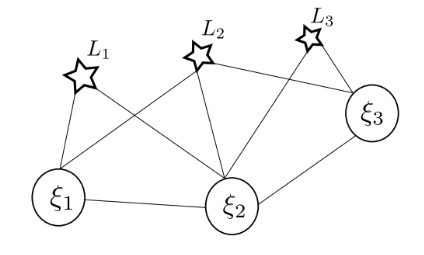
\includegraphics[width=0.7\textwidth]{1_1.png}    
\caption{相机位姿与路标点}
\label{img0}
\end{figure}
\indent 此处残差总共有9维;状态变量有3个相机pose,3个路标点坐标共六维;所以雅克比矩阵为$6\times9$维,信息矩阵为$6 \times 6$维。\\
\subsubsection{$\Lambda_1$}
\indent 记$r_1=r(\xi _1,\xi _2)$ \\
\begin{equation}
\begin{aligned}
&J_1= \begin{bmatrix}
    \frac{\partial r_1}{\partial \xi _1} & \frac{\partial r_1}{\partial \xi _2} &0 &0 &0 &0 
    \end{bmatrix}\\
&\Lambda_1=J_1^T\Sigma_1^{-1}J_1
\end{aligned}
\end{equation}

\subsubsection{$\Lambda_2$}
\indent 记$r_2=r(\xi _2,\xi _3)$ \\
\begin{equation}
\begin{aligned}
&J_2= \begin{bmatrix}
    0 & \frac{\partial r_2}{\partial \xi _2} &\frac{\partial r_2}{\partial \xi _3} &0 &0 &0 
    \end{bmatrix}\\
&\Lambda_2=J_2^T\Sigma_2^{-1}J_2
\end{aligned}
\end{equation}

\subsubsection{$\Lambda_3$}
\indent 记$r_3=r(\xi _1,L _1)$ \\
\begin{equation}
\begin{aligned}
&J_3= \begin{bmatrix}
     \frac{\partial r_3}{\partial \xi _1} &0 &0 &\frac{\partial r_3}{\partial L_1} &0 &0 
    \end{bmatrix}\\
&\Lambda_3=J_3^T\Sigma_3^{-1}J_3
\end{aligned}
\end{equation}

\subsubsection{$\Lambda_4$}
\indent 记$r_4=r(\xi _1,L _2)$ \\
\begin{equation}
\begin{aligned}
&J_4= \begin{bmatrix}
    \frac{\partial r_4}{\partial \xi _1} &0 &0 &0 &\frac{\partial r_4}{\partial L_2} &0 
    \end{bmatrix}\\
&\Lambda_4=J_4^T\Sigma_4^{-1}J_4
\end{aligned}
\end{equation}

\subsubsection{$\Lambda_5$}
\indent 记$r_5=r(\xi _2,L _1)$ \\
\begin{equation}
\begin{aligned}
&J_5= \begin{bmatrix}
    &0 &\frac{\partial r_5}{\partial \xi _2} &0  &\frac{\partial r_5}{\partial L_1} &0 &0
    \end{bmatrix}\\
&\Lambda_5=J_5^T\Sigma_5^{-1}J_5
\end{aligned}
\end{equation}

\subsubsection{$\Lambda_6$}
\indent 记$r_6=r(\xi _2,L _2)$ \\
\begin{equation}
\begin{aligned}
&J_6= \begin{bmatrix}
    &0 &\frac{\partial r_6}{\partial \xi _2} &0 &0 &\frac{\partial r_6}{\partial L_2} &0 
    \end{bmatrix}\\
&\Lambda_6=J_6^T\Sigma_6^{-1}J_6
\end{aligned}
\end{equation}

\subsubsection{$\Lambda_7$}
\indent 记$r_7=r(\xi _2,L _3)$ \\
\begin{equation}
\begin{aligned}
&J_7= \begin{bmatrix}
    &0 &\frac{\partial r_7}{\partial \xi _2} &0 &0 &0 &\frac{\partial r_7}{\partial L_3}  
    \end{bmatrix}\\
&\Lambda_7=J_7^T\Sigma_7^{-1}J_7
\end{aligned}
\end{equation}

\subsubsection{$\Lambda_8$}
\indent 记$r_8=r(\xi _3,L _2)$ \\
\begin{equation}
\begin{aligned}
&J_8= \begin{bmatrix}
    &0 &0 &\frac{\partial r_8}{\partial \xi _2} &0 &\frac{\partial r_8}{\partial L_2} &0 
    \end{bmatrix}\\
&\Lambda_8=J_8^T\Sigma_8^{-1}J_8
\end{aligned}
\end{equation}

\subsubsection{$\Lambda_9$}
\indent 记$r_9=r(\xi _3,L _3)$ \\
\begin{equation}
\begin{aligned}
&J_9= \begin{bmatrix}
    &0 &\frac{\partial r_9}{\partial \xi _2} &0 &0 &0 &\frac{\partial r_9}{\partial L_3}
    \end{bmatrix}\\
&\Lambda_9=J_9^T\Sigma_9^{-1}J_9
\end{aligned}
\end{equation}

\subsubsection{信息矩阵$\Lambda$}
\begin{figure}[H]
\centering
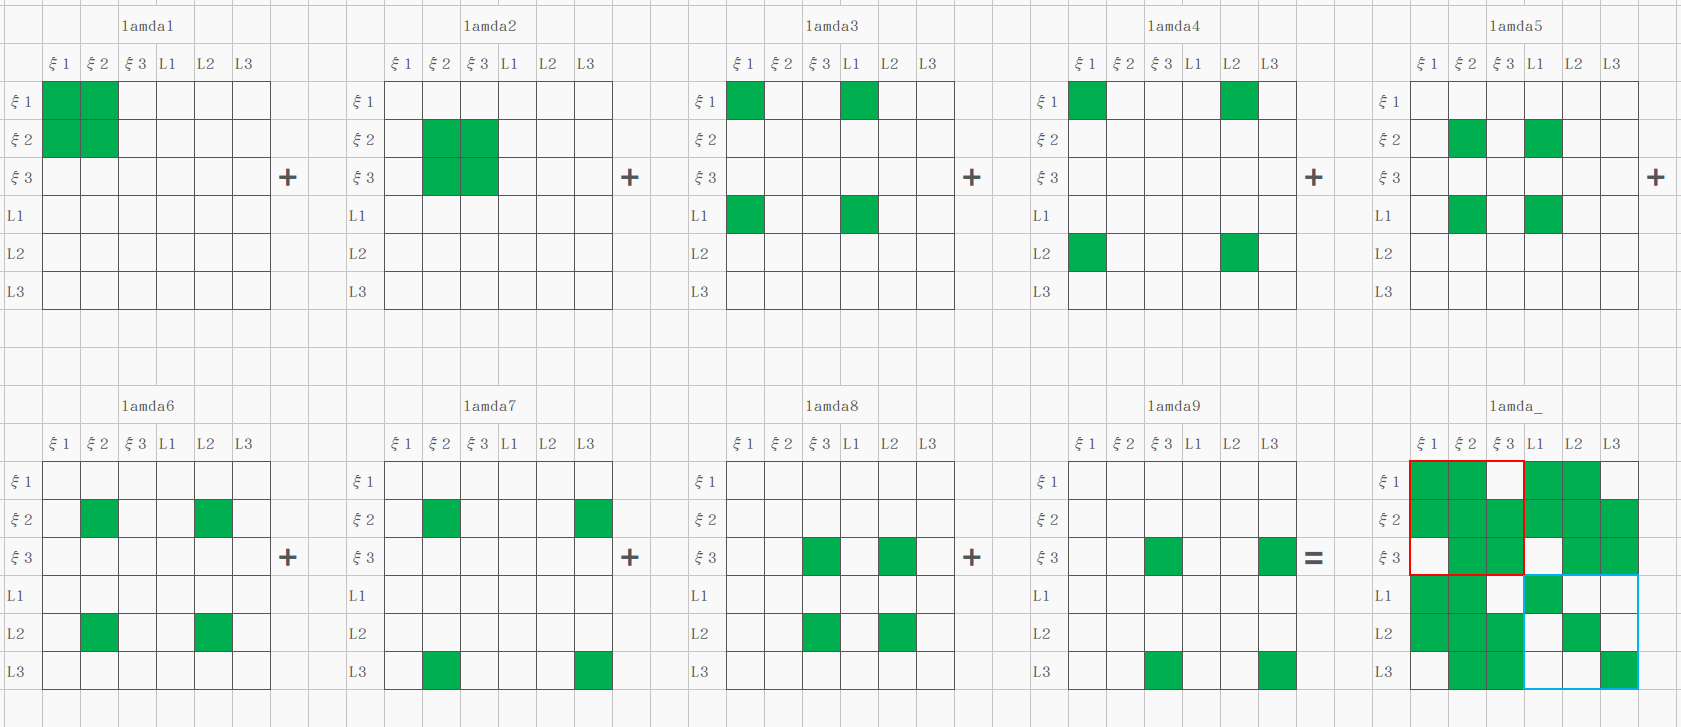
\includegraphics[width=1.1\textwidth]{1.1.png}    
\caption{信息矩阵}
\label{img1}
\end{figure}

\subsection{绘制相机位姿$\xi _1$被marg后的信息矩阵$\Lambda '$}
\begin{figure}[H]
\centering
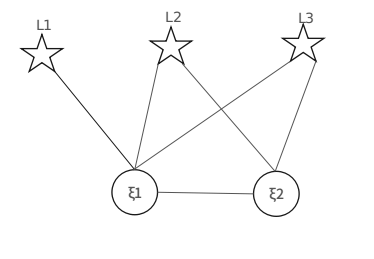
\includegraphics[width=0.7\textwidth]{1_2.png}    
\caption{marg后相机位姿与路标点}
\label{img1}
\end{figure}

\begin{figure}[H]
\centering
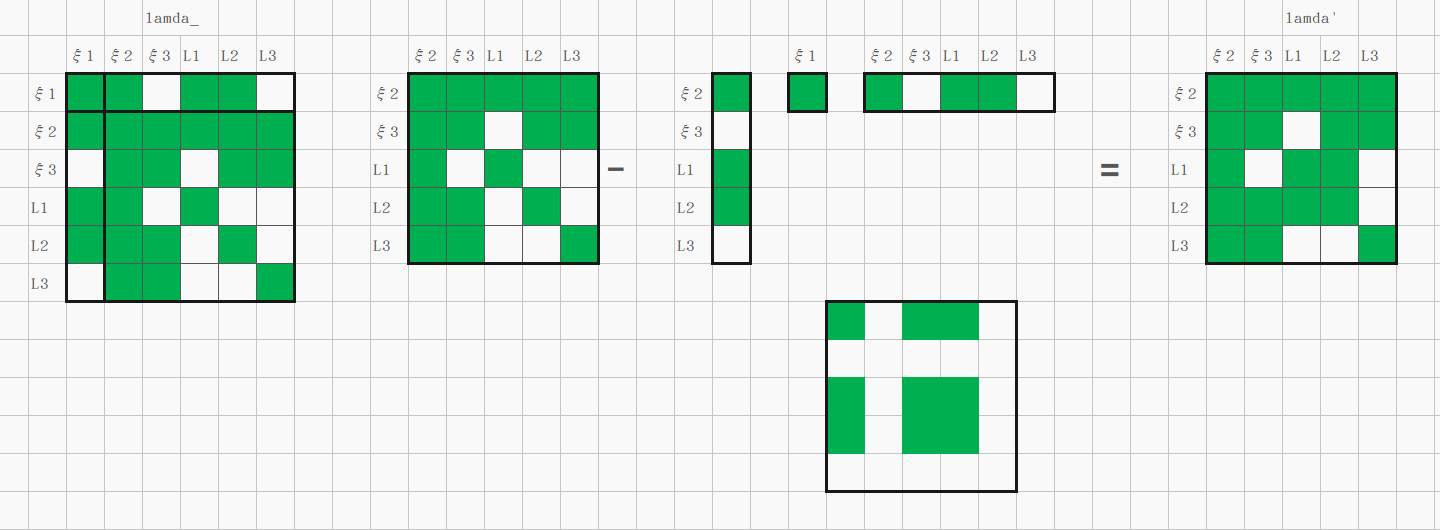
\includegraphics[width=1.1\textwidth]{1.2.png}    
\caption{marg后的信息矩阵}
\label{img1}
\end{figure}

\newpage
\section{代码补充}
\indent 补充代码中单目bundle adjustment信息矩阵计算部分。\\
\begin{lstlisting}[language={c++}]
    H.block(i*6,i*6,6,6) += jacobian_Ti.transpose() * jacobian_Ti;
    /// 请补充完整作业信息矩阵块的计算
    H.block(6*poseNums+j*3,6*poseNums+j*3,3,3) += jacobian_Pj.transpose() * jacobian_Pj;
    H.block(i*6,6*poseNums+j*3 , 6,3) += jacobian_Ti.transpose() * jacobian_Pj;
    
    H.block(j*3 + 6*poseNums,i*6 , 3,6) += jacobian_Pj.transpose() * jacobian_Ti;
\end{lstlisting}

\begin{figure}[H]
\centering
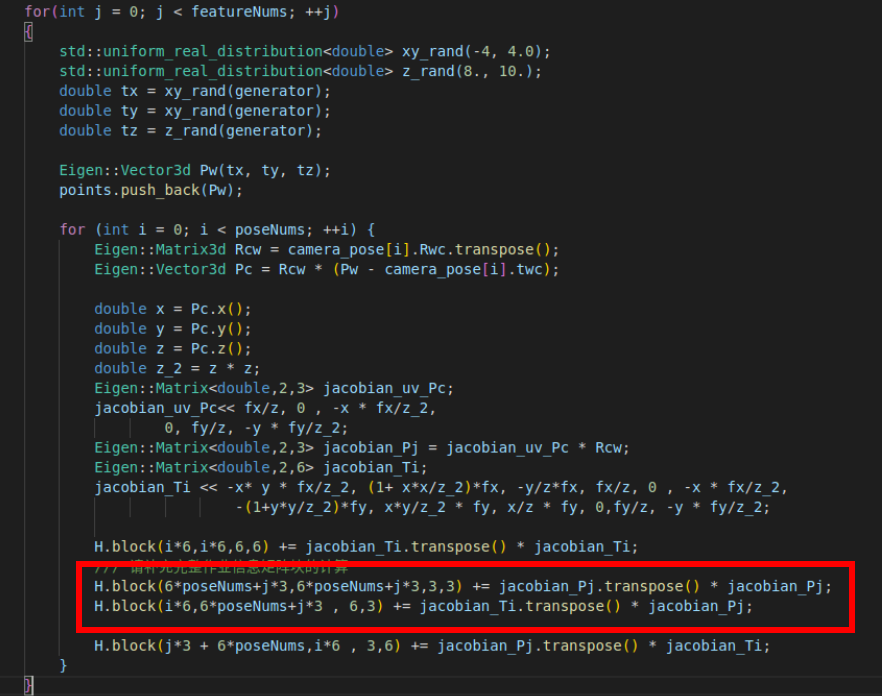
\includegraphics[width=0.7\textwidth]{2.1.1.png}    
\caption{信息矩阵计算补充}
\label{img1}
\end{figure}
\indent 信息矩阵SVD分解后结果:\\
\begin{figure}[H]
\centering
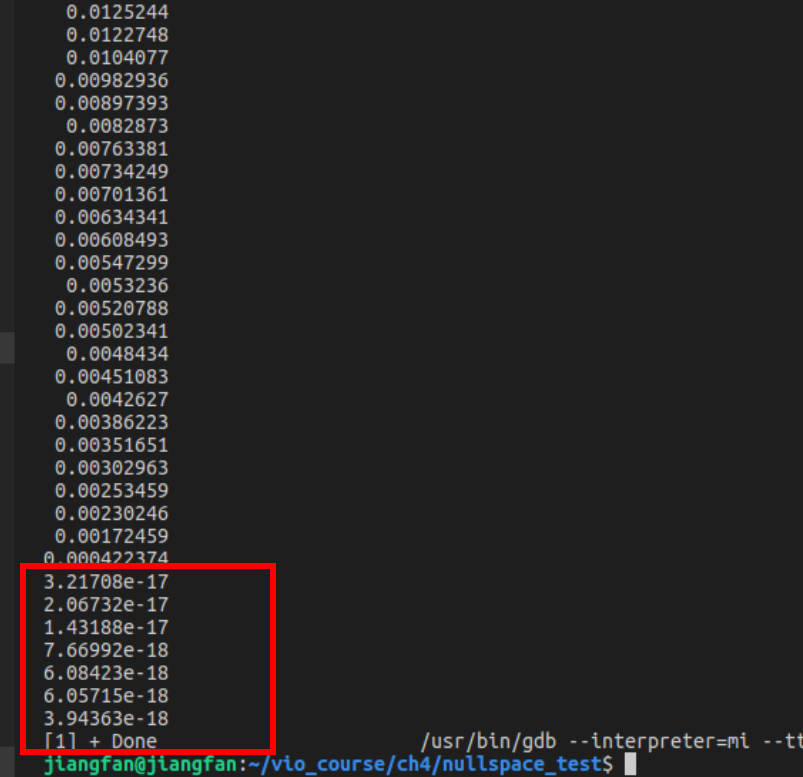
\includegraphics[width=0.6\textwidth]{2.1.2.png}    
\caption{信息矩阵SVD分解}
\label{img1}
\end{figure}
\indent 奇异值分解后从图上可以看出后七维接近于0,说明单目slam的BA求解零空间维度为7。
\end{document}